\subsection{Диаграмма вариантов использования}
\label{sec:tech-requirements:functional-model}

Функциональная модель системы описывает поведение разрабатываемого программного продукта с точки зрения различных ролей пользователей, участвующих во взаимодействии с системой. Одним из основных инструментов для визуализации функциональных возможностей системы является диаграмма вариантов использования, которая отражает связи между актёрами и прецедентами (сценариями взаимодействия с системой).

Исходя из общей архитектуры системы и анализа требований, были выделены три ключевые роли (актёра):

\begin{itemize}
    \item сотрудник~-- основной пользователь системы, осуществляющий бронирование ресурсов и взаимодействие с функционалом в рамках своей повседневной деятельности;
    \item офис-менеджер~-- ответственен за управление бронированием ресурсов, контроль наличия и состояния оборудования;
    \item менеджер по персоналу~-- осуществляет администрирование пользователей, контроль посещаемости и управление правами доступа.
\end{itemize}

Сотрудник~-- это зарегистрированный пользователь, работающий в офисе на постоянной или временной основе. Основной задачей для данной роли является эффективное планирование и использование офисных ресурсов. Сотрудник взаимодействует с системой через следующие прецеденты:

\begin{enumerate}
    \item Авторизация в системе~-- пользователь проходит процедуру входа с использованием логина и пароля;
    \item Просмотр доступных рабочих мест~-- пользователь получает список свободных мест по выбранным фильтрам (офис, этаж, тип зоны).
    \item Бронирование рабочего места~-- сотрудник выбирает конкретное место, дату и интервал времени, указывает предпочтения (например, ближе к окну).
    \item Просмотр статуса бронирований~-- система отображает активные, завершённые и отклонённые бронирования.
    \item Отмена бронирования рабочего места~-- пользователь имеет возможность отменить ранее созданное бронирование.
    \item Создание запроса на бронирование оборудования~-- формируется заявка на использование ноутбука, проектора или другого инвентаря.
    \item Просмотр расписания оборудования~-- сотрудник может увидеть, в какие дни и часы оборудование занято или свободно.
    \item Запрос на временный доступ в помещение~-- при необходимости доступа к закрытому кабинету или складу, сотрудник отправляет заявку.
    \item Получение уведомлений~-- система информирует о подтверждении/отклонении бронирований, изменениях доступа и других событиях.
    \item Просмотр отчёта о посещаемости~-- сотрудник может ознакомиться со своей историей входов и выходов из помещений.
\end{enumerate}

Диаграмма вариантов использования от имени сотрудника представлена на рис.~\ref{fig:tech-requirements:functional-model:use-cases-employee}.

\afterpage{
    \clearpage
    \begin{landscape}
        \thispagestyle{landscape}
        \begin{figure}[p]
            \centering
            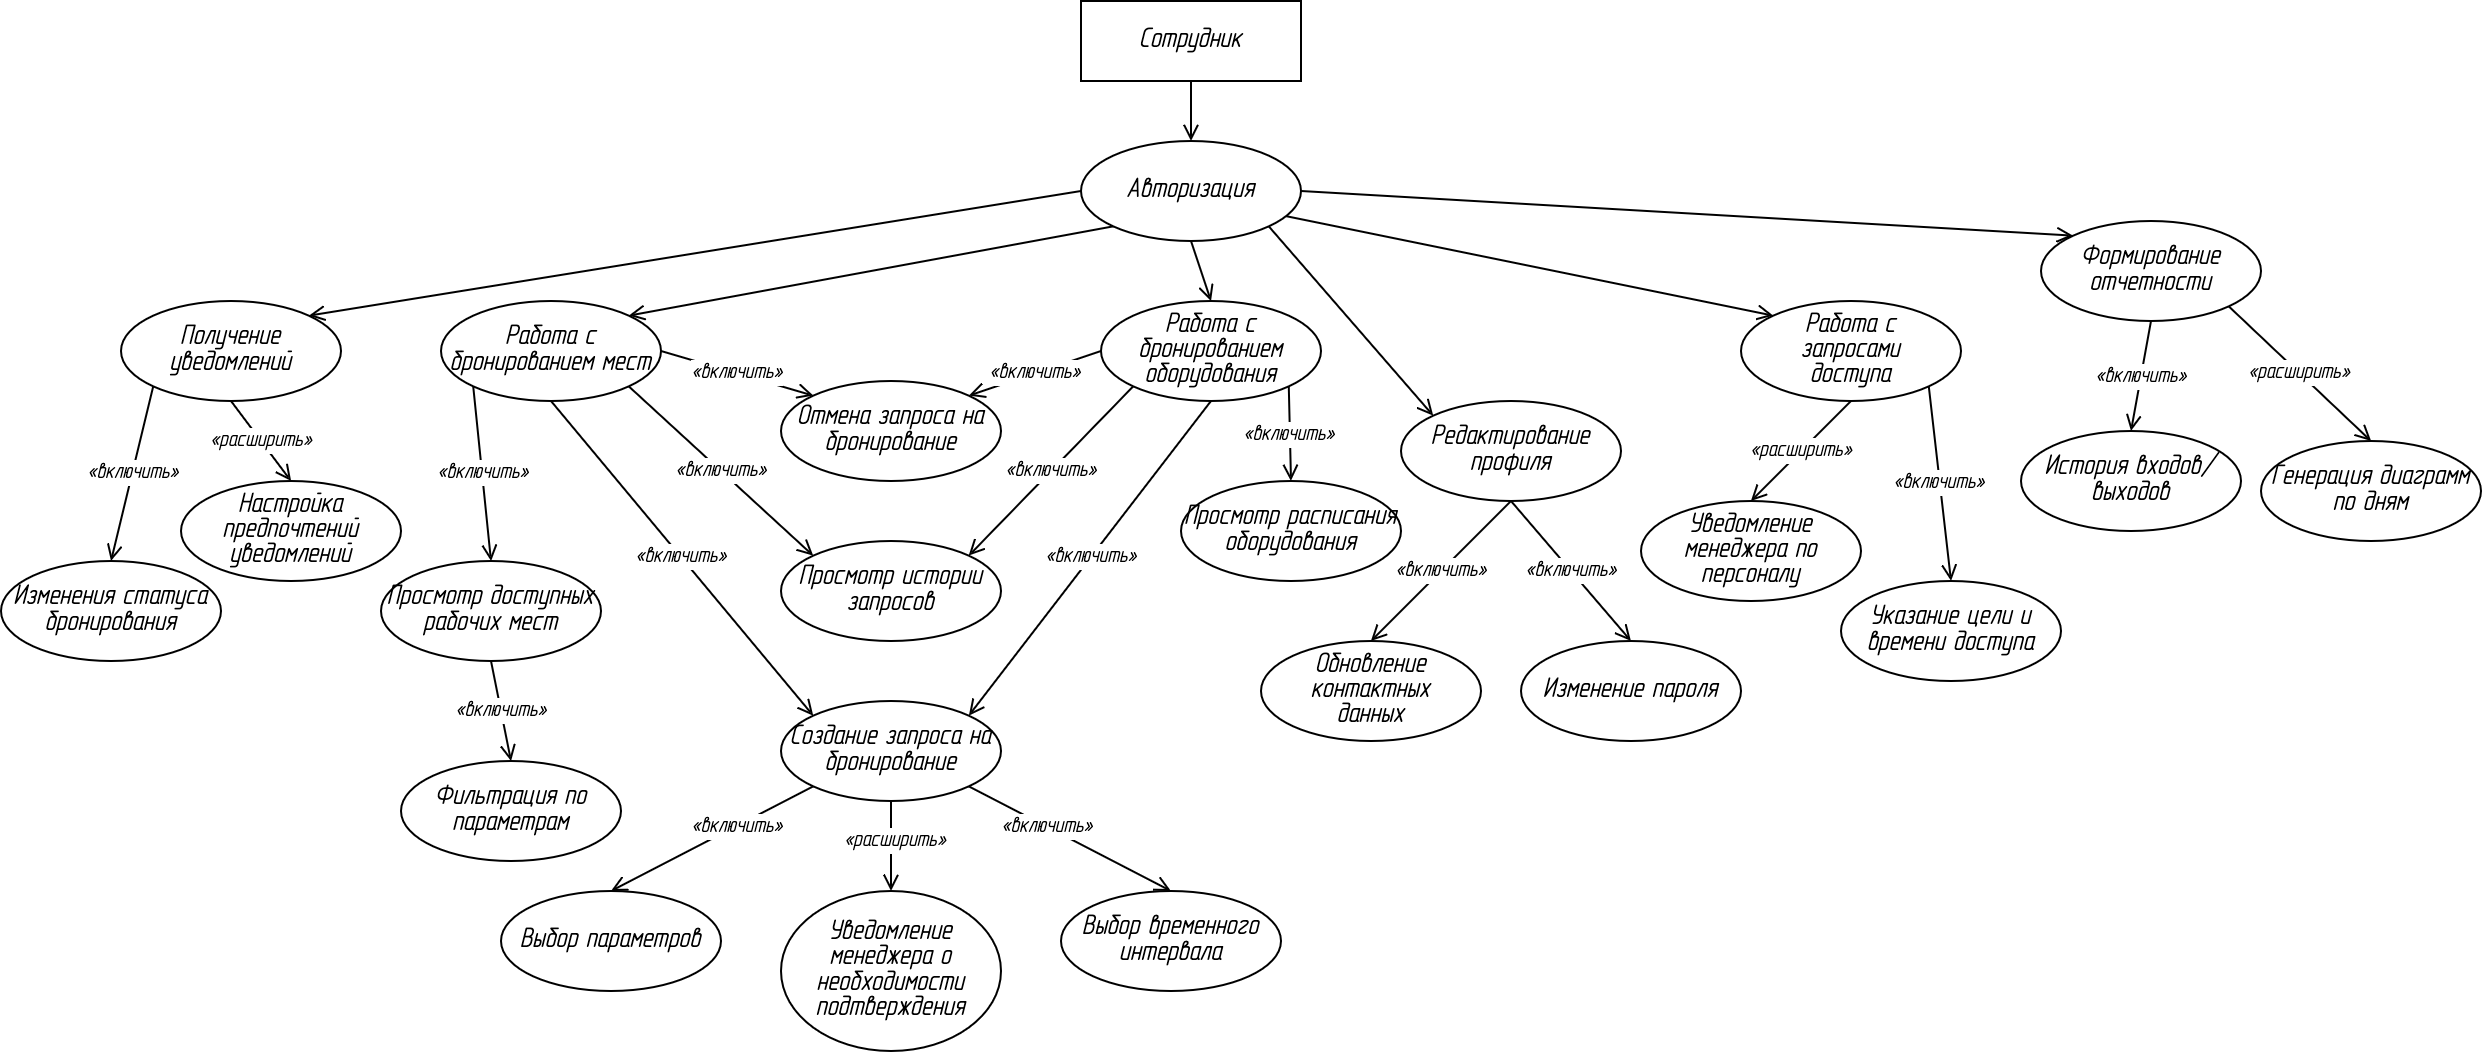
\includegraphics[width=0.99\linewidth]{assets/use-cases-employee.png}
            \caption{Диаграмма вариантов использования от имени сотрудника}
            \label{fig:tech-requirements:functional-model:use-cases-employee}
        \end{figure}
    \end{landscape}
    \clearpage
}

Актёр «Офис-менеджер» в рамках системы выполняет функции административного контроля и технической поддержки сотрудников. Основные задачи этой роли связаны с обработкой заявок на бронирование офисных ресурсов, контролем состояния оборудования и рабочих мест, управлением расписаниями и генерацией отчётности.

Офис-менеджер также после авторизации имеет доступ к набору определенных функций, соответствующих его роли.

\begin{enumerate}
    \item \textit{Обработка заявок на бронирование}~-- ключевая функция офис-ме\-нед\-же\-ра, в рамках которой он получает, просматривает и обрабатывает заявки, созданные сотрудниками на бронирование ресурсов:
    \begin{itemize}
        \item просмотр входящих заявок~-- система предоставляет список всех новых и активных заявок на бронирование;
        \item подтверждение бронирования рабочего места~-- одобрение запроса на использование конкретного рабочего места;
        \item подтверждение бронирования оборудования~-- аналогичная функция для инвентаря, например, ноутбуков или проекторов;
        \item уведомление сотрудника о принятом решении~-- система автоматически отправляет уведомление пользователю с информацией об одобрении или отклонении его запроса.
    \end{itemize}
    
    \item \textit{Контроль состояния ресурсов} позволяет офис-менеджеру анализировать текущее состояние всех доступных офисных ресурсов, чтобы управлять ими эффективно:
    \begin{itemize}
        \item просмотр карты офиса~-- визуальный интерфейс с расположением этажей, комнат, рабочих мест и их статусами;
        \item проверка статуса оборудования~-- отображение данных о доступности, использовании, поломках и других параметрах техники;
        \item вывод отчётов по использованию~-- генерация сводной статистики по загруженности офисных ресурсов.
    \end{itemize}

    \item \textit{Редактирование параметров ресурсов} позволяет вносить изменения в описание и характеристики ресурсов, управлять их видимостью и статусом:
    \begin{itemize}
        \item изменение характеристик рабочих мест и оборудования;
        \item добавление новых ресурсов~-- используется, когда в систему добавляется новый инвентарь или офисное пространство (например, после переоснащения).
    \end{itemize}

    \item \textit{Управление календарями бронирования}~-- офис-менеджер управляет графиками доступности офисных помещений и оборудования, учитывая внутренние мероприятия, ремонты и профилактику:
    \begin{itemize}
        \item блокировка недоступных интервалов~-- для указания времени, когда ресурс будет недоступен;
        \item установка расписаний обслуживания~-- например, регулярное техобслуживание оборудования.
    \end{itemize}

    \item \textit{Генерация отчётов по бронированиям} позволяет офис-менеджеру формировать отчёты об использовании ресурсов по различным критериям: по сотрудникам, помещениям, временным интервалам и т.д.
    \begin{itemize}
        \item формирование отчётов;
        \item автоматическая отправка отчётов менеджеру по персоналу~-- интеграция между ролями в рамках одной информационной системы;
    \end{itemize}

    \item \textit{Управление уведомлениями} с возможностью настройки шаблонов и каналов доставки уведомлений о событиях в системе: новых заявках, изменениях статусов, напоминаниях и т.д.
    \begin{itemize}
        \item настройка шаблонов уведомлений~-- редактор текстов сообщений;
        \item управление каналами доставки~-- выбор между электронной почтой, \textit{push}-уведомлениями, \textit{SMS} и др.
    \end{itemize}
\end{enumerate}

Диаграмма вариантов использования от имени офис-менеджера представлена на рис.~\ref{fig:tech-requirements:functional-model:use-cases-office_manager}.

\afterpage{
    \clearpage
    \begin{landscape}
        \thispagestyle{landscape}
        \begin{figure}[p]
            \centering
            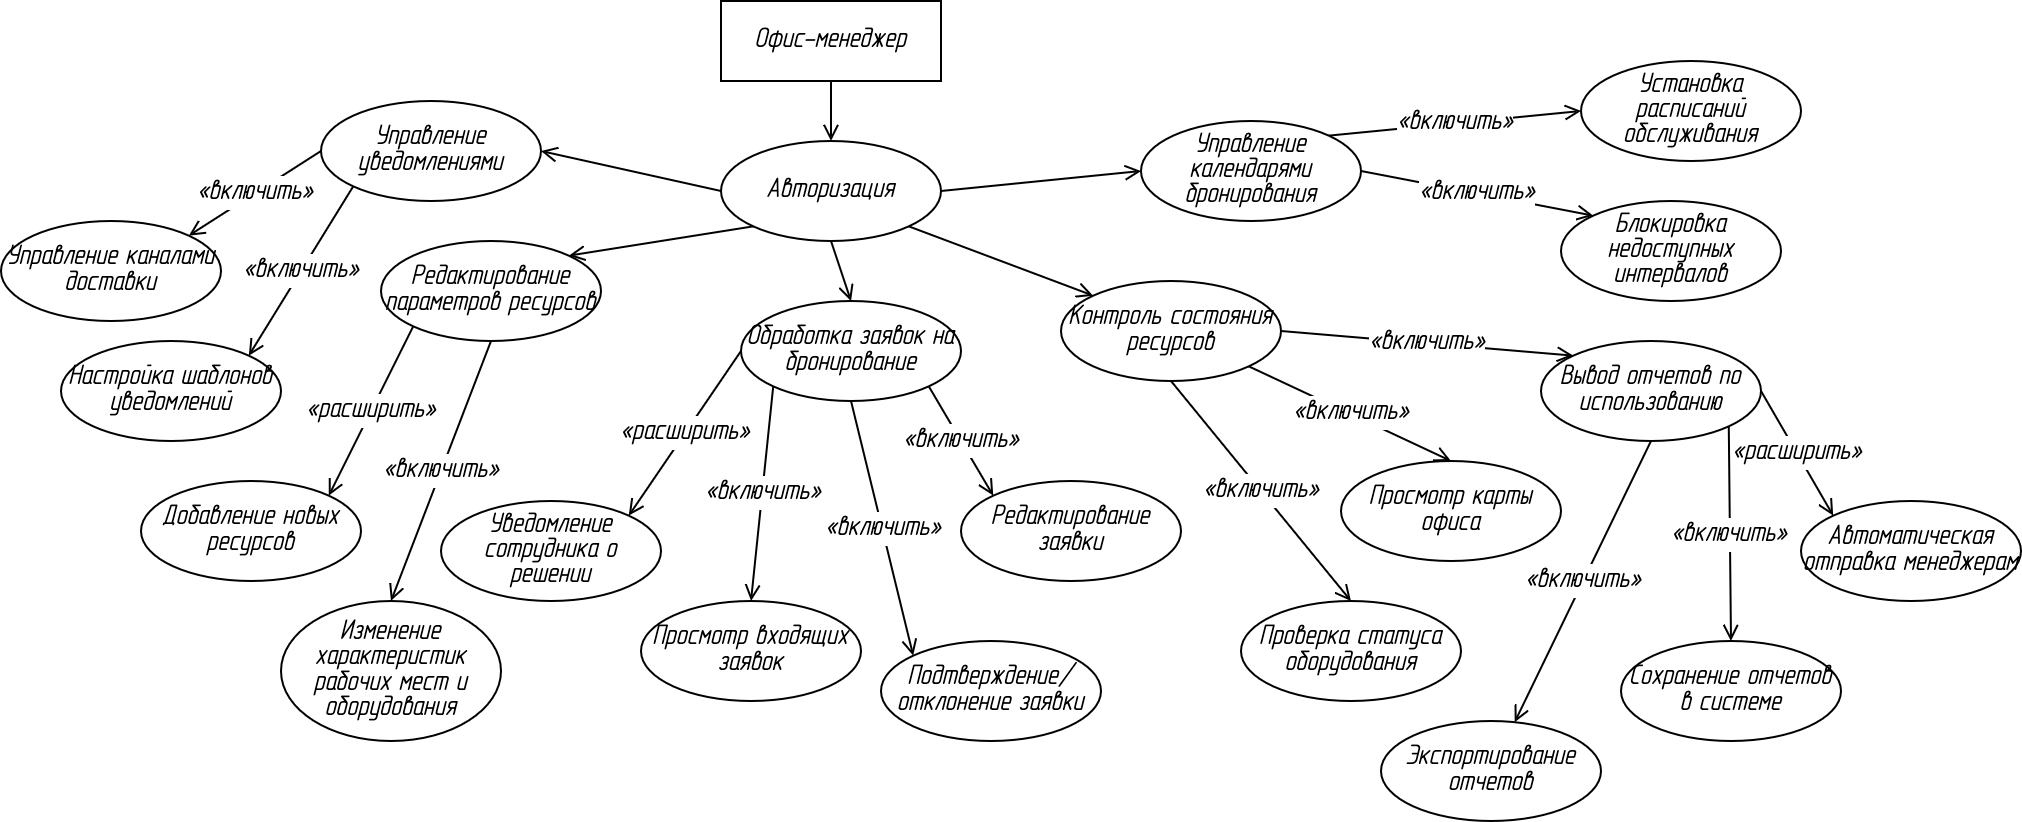
\includegraphics[width=0.99\linewidth]{assets/use-cases-office_manager.png}
            \caption{Диаграмма вариантов использования от имени офис-менеджера}
            \label{fig:tech-requirements:functional-model:use-cases-office_manager}
        \end{figure}
    \end{landscape}
    \clearpage
}
